\documentclass[12pt, a4paper]{article}

% --- Packages ---
\usepackage[utf8]{inputenc}
\usepackage[T1]{fontenc}
\usepackage[french]{babel}
\usepackage{graphicx}
\usepackage{fancyhdr}
\usepackage{geometry}
\usepackage{titlesec}
\usepackage{hyperref}
\usepackage{float} % <--- AJOUTÉ pour l'option [H]

% --- Configuration des marges ---
\geometry{margin=2.5cm, headheight=2cm}

% --- Configuration En-tête et Pied de Page ---
\pagestyle{fancy}
\fancyhf{}
\fancyhead[R]{
\includegraphics[height=1cm]{logo_upssitech.png}} 
\fancyfoot[L]{Victor Chalumeaux} 
\fancyfoot[R]{\thepage}
\renewcommand{\headrulewidth}{0.5pt}

\begin{document}

% --- Page de Garde ---
\begin{titlepage}
    \thispagestyle{empty} 
    \noindent 
    \begin{minipage}[t]{0.3\textwidth}
        \flushleft
        
\includegraphics[width=\textwidth]{logo_upssitech.png} 
    \end{minipage}
    \hfill
    \begin{minipage}[t]{0.3\textwidth}
        \flushright
        
\includegraphics[width=\textwidth]{logo_sri.png} 
    \end{minipage}
    
    \vspace{2cm}
    
    \centering
    {\Huge \textbf{Rapport de Projet \newline La Course des Pirates}}\\[1cm]
    {\Large Développement d'Application Orienté Objet}\\[1cm]
    
    
\includegraphics[width=0.6\textwidth]{pirates.png} \\[0cm]
    
    \vfill
    {\large Présenté par : \textbf{Victor Chalumeaux}}\\[0.5cm]
    {\large Enseignant : Mr. Vanderstraeten}\\[1cm]
    {\large Date : \today}
\end{titlepage}

\newpage
\tableofcontents
\newpage

% --- Section 1 : Architecture ---
\section{Architecture et Conception}
L'un des objectifs majeurs de ce projet a été la stricte séparation entre la \textbf{logique métier} (le Modèle) et les \textbf{interactions utilisateurs} (la Vue).

\subsection{Séparation Modèle / Affichage}
Le projet est structuré en deux entités distinctes pour garantir une meilleure maintenabilité :
\begin{itemize}
    \item \textbf{Le package \texttt{jeu}} : Il contient les règles de mouvement, la gestion du plateau et l'état des pirates.
    \item \textbf{Le package \texttt{journaldebord}} : Via la classe \texttt{Narrateur}, il gère l'affichage.
\end{itemize}

\begin{figure}[H] % <--- CHANGÉ EN [H]
    \centering
    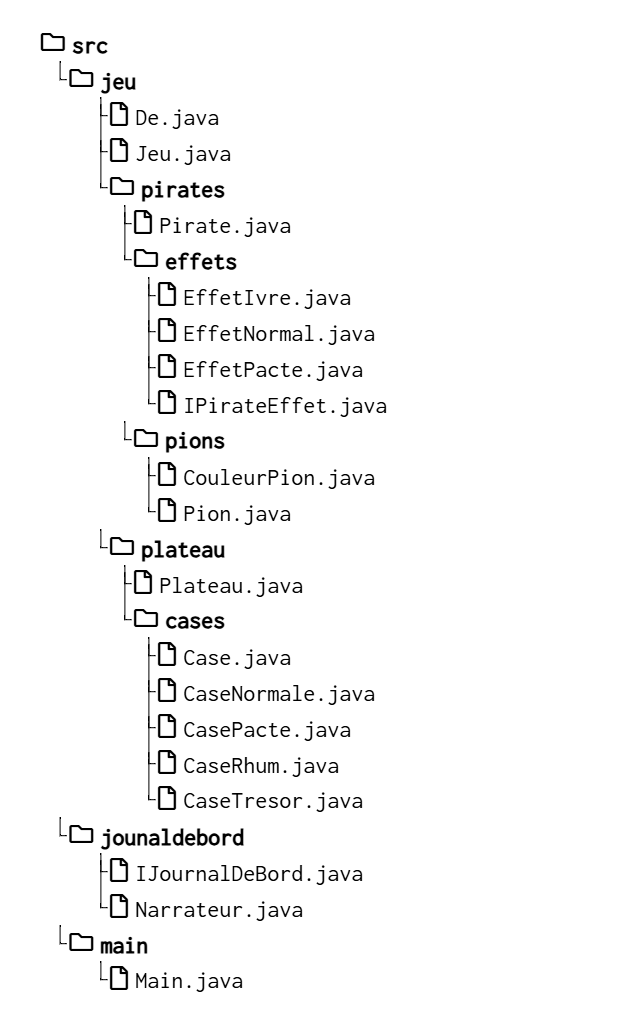
\includegraphics[width=0.4\textwidth]{project_structure.png}
    \caption{Structure de l'arborescence du projet}
\end{figure}

\subsection{Respect des contraintes techniques}
Conformément aux consignes, aucune collection n'a été utilisée. Le code a été audité via l'outil \textbf{SonarLint}.

% --- Section 2 : Diagramme de Séquence Système ---
\newpage
\section{Diagramme de Séquence Système}
Le diagramme suivant illustre le déroulement global d'une partie.

\begin{figure}[H] % <--- CHANGÉ EN [H]
    \centering
    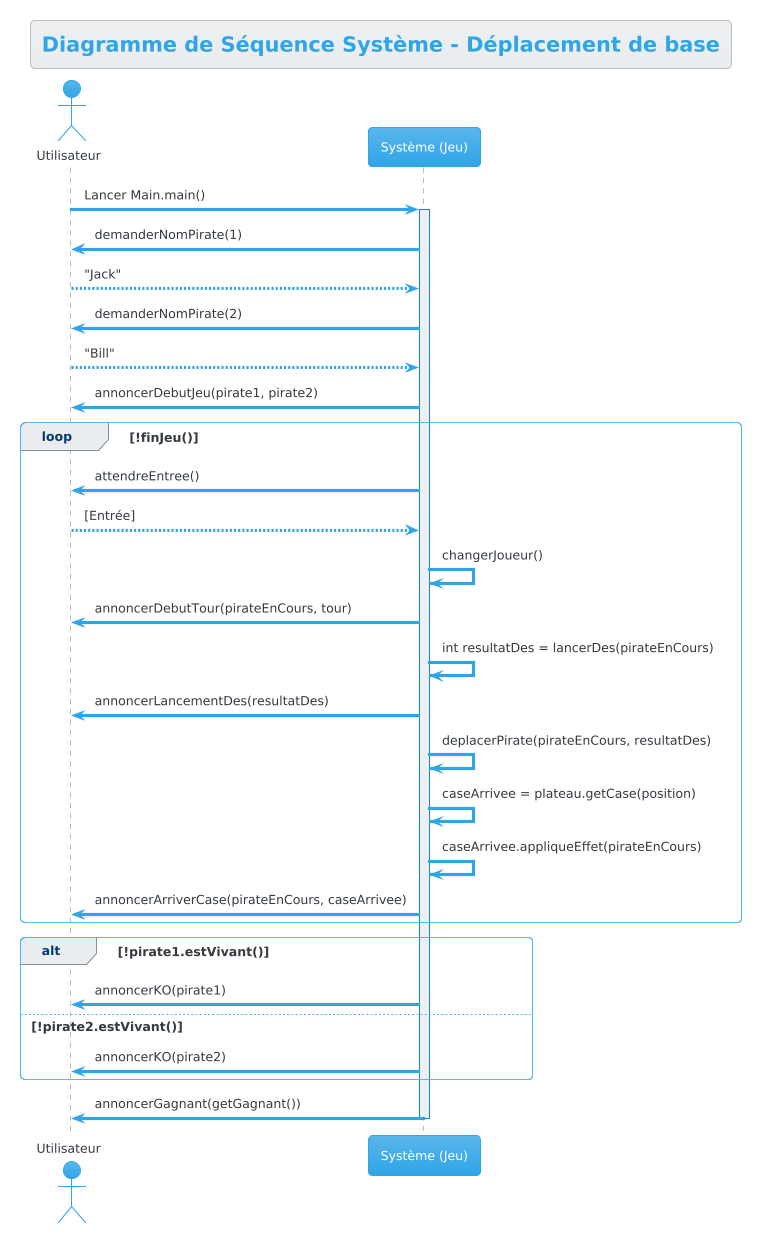
\includegraphics[width=0.7\textwidth]{UML_sequence_system.png}
    \caption{Interaction entre l'utilisateur et le moteur de jeu}
\end{figure}

\textbf{Commentaire :} L'appel \texttt{lancerDes(pirateEnCours)} encapsule toute la complexité du calcul de déplacement.

% --- Section 3 : Conception Détaillée ---
\newpage
\section{Conception Détaillée du Modèle}

\subsection{Architecture Globale}
Ce diagramme présente les relations de haut niveau entre les composants.

\begin{figure}[H] % <--- CHANGÉ EN [H]
    \centering
    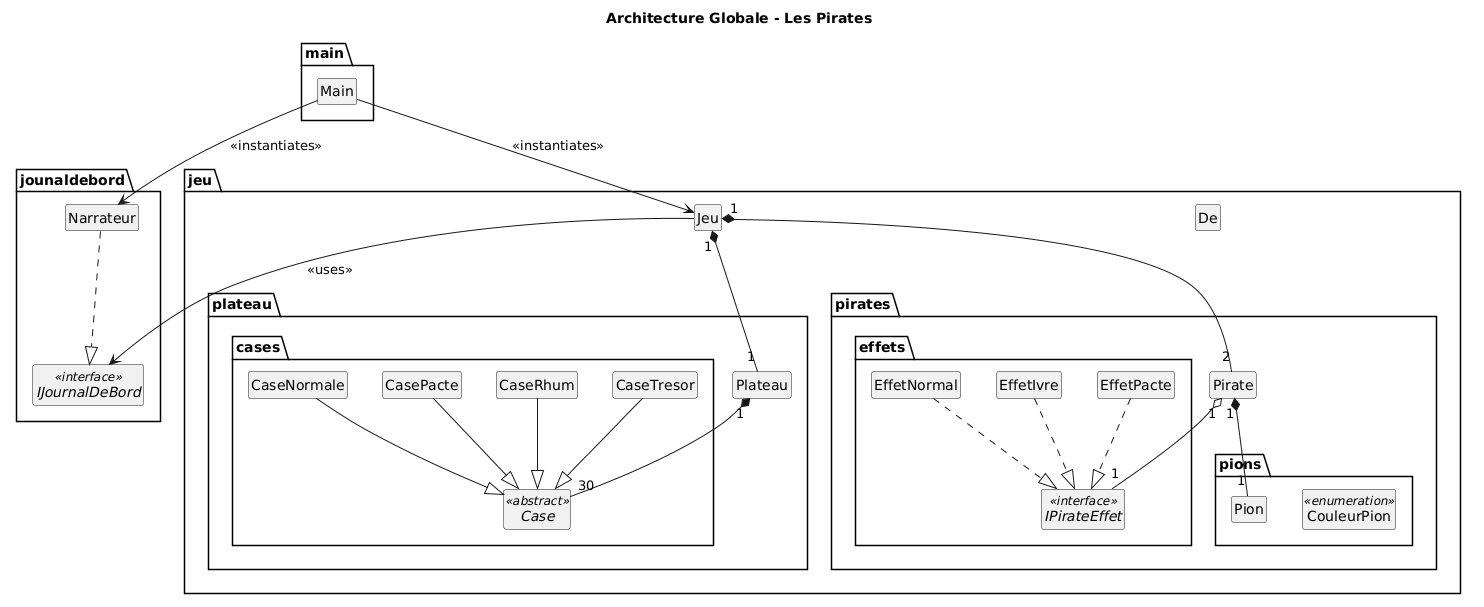
\includegraphics[width=0.8\textwidth]{UML_objects_global.png} 
    \caption{Vue d'ensemble de l'architecture logicielle}
\end{figure}

\subsection{Structure du package \texttt{jeu.pirates}}
Ce diagramme détaille la gestion des entités et de leurs états. Le \texttt{Pirate} délègue la logique de calcul de son mouvement à l'interface \texttt{IPirateEffet}, ce qui permet de modifier son comportement dynamiquement sans changer le code de la classe \texttt{Pirate}.

\begin{figure}[H] % <--- CHANGÉ EN [H]
    \centering
    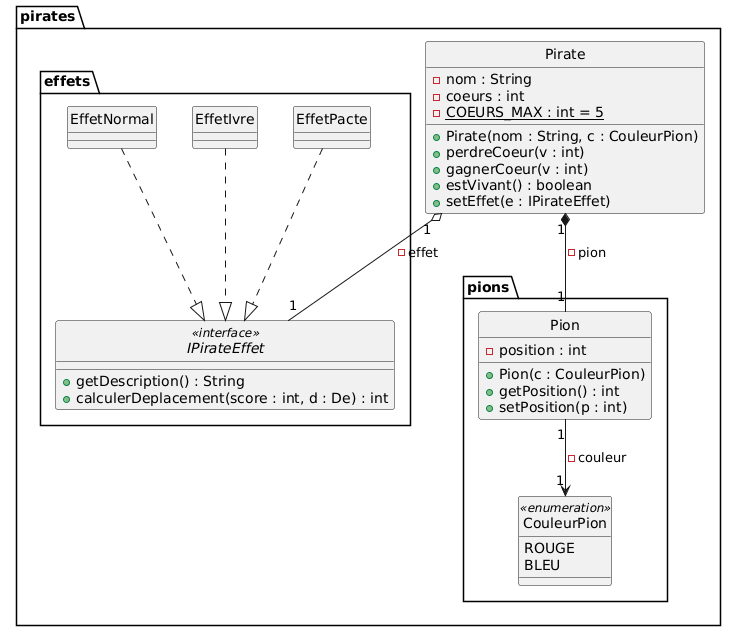
\includegraphics[width=0.6\textwidth]{UML_objects_pirates.png} 
    \caption{Diagramme des classes liées aux pirates}
\end{figure}

\subsection{Structure du package \texttt{jeu.plateau}}
Le plateau est composé d'un tableau fixe de 30 cases. L'utilisation d'une classe abstraite \texttt{Case} permet d'implémenter le \textbf{polymorphisme}.

\begin{figure}[H] % <--- CHANGÉ EN [H]
    \centering
    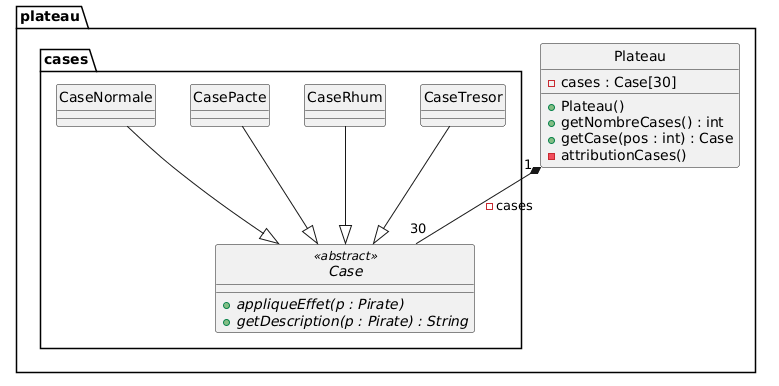
\includegraphics[width=0.6\textwidth]{UML_objects_plateau.png} 
    \caption{Hiérarchie des cases et structure du plateau}
\end{figure}

Cette architecture permet de distinguer plusieurs types de comportements lors de l'arrivée d'un pion sur une case :

\begin{itemize}
    \item \textbf{CaseNormale} : Cette case agit comme une zone neutre. Elle réinitialise le comportement du pirate pour que son prochain déplacement soit standard.
    
    \item \textbf{CaseRhum} : Le pirate récupère 1 point de vie en tombant sur cette case. En contrepartie, il subit un malus d'ébriété qui le forcera à reculer des son résultat lors de son prochain tour de jeu.

    \item \textbf{CasePacte} : Le pirate sacrifie 2 points de vie pour conclure un pacte sombre. Ce sacrifice lui permet de lancer un dé en plus lors de son prochain tour.

    \item \textbf{CaseTresor} : Située à la 30\textsuperscript{ème} et dernière position du plateau, cette case ne possède aucun effet sur les statistiques du pirate. Elle sert de marqueur de victoire pour désigner le gagnant de la partie.
\end{itemize}

\subsection{Structure du package \texttt{jeu.journaldebord}}
Ce package isole totalement la console du reste du code.

\begin{figure}[H] % <--- CHANGÉ EN [H]
    \centering
    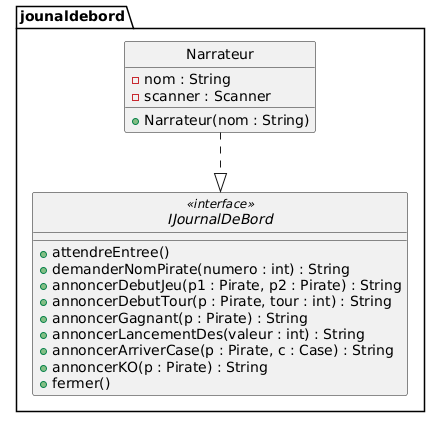
\includegraphics[width=0.6\textwidth]{UML_objects_journaldebord.png} 
    \caption{Diagramme des classes du journal de bord}
\end{figure}

% --- Section 4 : Dynamique des effets ---
\newpage
\section{Focus sur les effets spécifiques}
%
\subsection{Activation de la Case Rhum}

\end{document}